\documentclass{report}

\usepackage{listings}
\usepackage{polski}
\usepackage[utf8]{inputenc}
\usepackage[margin=1in]{geometry}
\usepackage[english,polish]{babel}\usepackage{indentfirst}
\usepackage[T1]{fontenc}
\usepackage{xcolor}
\usepackage{graphicx}
\usepackage{longtable}

% Default fixed font does not support bold face
\DeclareFixedFont{\ttb}{T1}{txtt}{bx}{n}{12} % for bold
\DeclareFixedFont{\ttm}{T1}{txtt}{m}{n}{12}  % for normal

% Custom colors
\usepackage{color}
\definecolor{deepblue}{rgb}{0,0,0.5}
\definecolor{deepred}{rgb}{0.6,0,0}
\definecolor{deepgreen}{rgb}{0,0.5,0}
\newcommand\pythonstyle{\lstset{
language=Python,
basicstyle=\ttm,
otherkeywords={self},             % Add keywords here
keywordstyle=\ttb\color{deepblue},
emph={MyClass,__init__},          % Custom highlighting
emphstyle=\ttb\color{deepred},    % Custom highlighting style
stringstyle=\color{deepgreen},
frame=tb,                         % Any extra options here
showstringspaces=false            %
}}

% Python environment
\lstnewenvironment{python}[1][]
{
\pythonstyle
\lstset{#1}
}
{}

% Python for external files
\newcommand\pythonexternal[2][]{{
\pythonstyle
\lstinputlisting[#1]{#2}}}

% Python for inline
\newcommand\pythoninline[1]{{\pythonstyle\lstinline!#1!}}

%\pagecolor{black}
%\color{white}

%\documentclass[eng]{mgr}
\usepackage{polski}
\usepackage[utf8]{inputenc}
%\usepackage{xcolor}
\usepackage[T1]{fontenc}

%pakiety do grafiki
\usepackage{graphicx}
\usepackage{psfrag}

%Wspomaganie tabel
\usepackage{array}
%\usepackage{tabularx}
\usepackage{hhline}
\usepackage{longtable}
%Matematyka
\usepackage{amsmath}
\usepackage{amsfonts}
\usepackage{hyperref}
\usepackage{float}
%pakiet wypisujący na marginesie etykiety równań„ i rysunkóww zdefiniowanych przez \label{}, chcąc wygenerować finalną wersję dokumentu wystarczy usunąć poniższą linię
%\usepackage{showlabels}
%\newcommand{\R}{I\!\!R} %symbol liczb rzeczywistych,
%\newtheorem{theorem}{Twierdzenie}[section] %nowe otoczenie do składania twierdzenia
\usepackage{subcaption}
\usepackage{fancyref}

\newenvironment{tightitemize}{\itemize\addtolength{\itemsep}{-5pt}}{\enditemize}

\title{Zastosowanie sztucznych sieci neuronowych do diagnostyki stanów ostrego brzucha}
\engtitle{Application of artificial neural networks to the diagnosis of surgical abdomen states}
\author{Mateusz Burniak}
\supervisor{prof. dr hab. inż. Marek Kurzyński \\ Katedra Systemów i Sieci Komputerowych}
\field{Informatyka (INF)}
\specialisation{Systemy informatyki w medycynie (IMT)}


% listings
\usepackage{listings}
% Default fixed font does not support bold face
\DeclareFixedFont{\ttb}{T1}{txtt}{bx}{n}{12} % for bold
\DeclareFixedFont{\ttm}{T1}{txtt}{m}{n}{12}  % for normal

% Custom colors
\usepackage{color}
\definecolor{deepblue}{rgb}{0,0,0.5}
\definecolor{deepred}{rgb}{0.6,0,0}
\definecolor{deepgreen}{rgb}{0,0.5,0}

\newcommand\pythonstyle{\lstset{
language=Python,
basicstyle=\ttm,
otherkeywords={self},             % Add keywords here
keywordstyle=\ttb\color{deepblue},
emph={MyClass,__init__},          % Custom highlighting
emphstyle=\ttb\color{deepred},    % Custom highlighting style
stringstyle=\color{deepgreen},
frame=tb,                         % Any extra options here
showstringspaces=false            %
}}


% Python environment
\lstnewenvironment{python}[1][]
{
\pythonstyle
\lstset{#1}
}
{}

% Python for external files
\newcommand\pythonexternal[2][]{{
\pythonstyle
\lstinputlisting[#1]{#2}}}

% Python for inline
\newcommand\pythoninline[1]{{\pythonstyle\lstinline!#1!}}


\begin{document}
    %    \maketitle
    \tableofcontents

    \chapter{Wstęp}\label{ch:wstęp}

    \section{Cel projektu}\label{sec:celProjektu}

    \section{Motywacja}\label{sec:motywacja}

    \chapter{Problem medyczny}\label{ch:problemMedyczny}

    Wybrany przeze mnie problem medyczny dotyczy klasyfikacji stanów ostrego brzucha.
    Za ten stan odpowiedzialne mogą być różne choroby, które zawsze wymagają interwejcji lekarza.
    % http://www.poradnikzdrowie.pl/zdrowie/uklad-pokarmowy/ostry-brzuch-przyczyny-objawy-leczenie-ostrego-brzucha_35445.html

    \section{Opis chorób}\label{sec:opisChorób}

    Do klasyfikacji jest 8 chorób, zatem sieć neuronowa będzie miała za zadanie przypisać 1 z 8 klas.
    Są to:
    \begin{enumerate}
        \item Ostre zapalenie wyrostka robaczkowego,
        \item Zapalenie uchyłków jelit,
        \item Niedrożność mechaniczna jelit,
        \item Perforowany wrzód trawienny,
        \item Zapalenie woreczka żółciowego,
        \item Ostre zapalenie trzustki,
        \item Niecharakterystyczny ból brzucha,
        \item Inne przyczyny ostrego bólu brzucha.
    \end{enumerate}

    \begin{figure}[h]
        \centering
        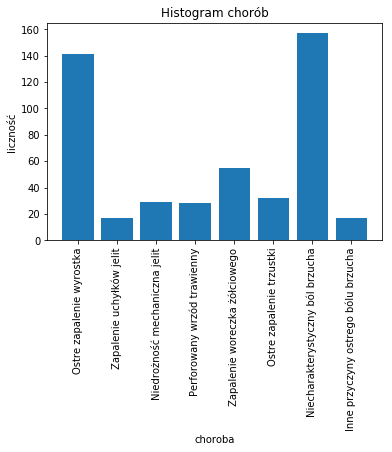
\includegraphics[scale=0.7]{./img/histogram.png}
        \caption{Histogram występowania chorób}
        %        \label{}
    \end{figure}

    Histogram pokazuje, że rozkład klas jest nierównomierny.
    Na 476 obiektów aż 157 to „Niecharakterystyczny ból brzucha” i 141 ma etykietę „Ostre zapalenie wyrostka robaczkowego”.
    Czyli do 2 klas należy ponad 60\% obiektów.
    Może to mieć negatywny wpływ na jakość klasyfikacji.

    \section{Opis cech}\label{sec:opisCech}

    Dane do tego problemu zawierają 31 cech.
    Są to odpowiedzi z wywiadu medycznego i wyniki przeprowadzonych badań.
    Możliwe wartości parametrów przedstawione są poniżej.
    Jak widać wszystkie liczby są naturalne mniejsze niż 11, także normalizacja czy skalowanie danych nie jest konieczne.

    
\begin{longtable}{|c|l|l|}
    \caption{Wszystkie cechy z odpowiedziami}\\ \hline
    \textbf{L.p.} & \textbf{Pytanie} & \textbf{Możliwe odpowiedzi} \\ \hline
    \endfirsthead
    \multicolumn{3}{c}
    {\tablename\ \thetable\ -- \textit{Wszystkie cechy z odpowiedziami - c.d.}} \\ \hline
    \textbf{L.p.} & \textbf{Pytanie} & \textbf{Możliwe odpowiedzi} \\ \hline
    \endhead
    \hline \multicolumn{3}{r}{\textit{Kontynuacja na następnej stronie}} \\
    \endfoot
    \hline
    \endlastfoot

\multicolumn{3}{|c|}{Ogólne} \\ \hline
1 & Płeć & \begin{tabular}[c]{l}1) męska  \\ 2) żeńska \end{tabular} \\ \hline
2 & Wiek & \begin{tabular}[c]{l}1) poniżej 20 lat  \\ 2) 20 - 30 lat  \\ 3) 21 - 30 lat  \\ 4) 31 - 40 lat  \\ 5) 41 - 50 lat  \\ 6) powyżej 50 lat \end{tabular} \\ \hline
\multicolumn{3}{|c|}{Ból} \\ \hline
3 & Lokalizacja bólu na początku zachorowania & \begin{tabular}[c]{l}1) prawa górna ćwiartka  \\ 2) lewa górna ćwiartka  \\ 3) górna połowa  \\ 4) prawa połowa  \\ 5) lewa połowa  \\ 6) centralny kwadrat  \\ 7) cały brzuch  \\ 8) prawa dolna ćwiartka  \\ 9) lewa dolna ćwiartka  \\ 10) dolna połowa \end{tabular} \\ \hline
4 & Lokalizacja bólu obecnie & \begin{tabular}[c]{l}0) brak bólu  \\ 1) prawa górna ćwiartka  \\ 2) lewa górna ćwiartka  \\ 3) górna połowa  \\ 4) prawa połowa  \\ 5) lewa połowa  \\ 6) centralny kwadrat  \\ 7) cały brzuch  \\ 8) prawa dolna ćwiartka  \\ 9) lewa dolna ćwiartka  \\ 10) dolna połowa \end{tabular} \\ \hline
5 & Intensywność bólu & \begin{tabular}[c]{l}0) łagodny/brak  \\ 1) umiarkowany  \\ 2) silny \end{tabular} \\ \hline
6 & Czynniki nasilające ból & \begin{tabular}[c]{l}0) brak czynników  \\ 1) oddychanie  \\ 2) kaszel  \\ 3) ruchy ciała \end{tabular} \\ \hline
7 & Czynniki przynoszące ulgę & \begin{tabular}[c]{l}0) brak czynników  \\ 1) wymioty  \\ 2) pozycja ciała \end{tabular} \\ \hline
8 & Progresja bólu & \begin{tabular}[c]{l}1) ustepujący  \\ 2) bez zmian  \\ 3) nasilający się \end{tabular} \\ \hline
9 & Czas trwania bólu & \begin{tabular}[c]{l}1) mniej niż 12 godzin  \\ 2) 12 - 24 godzin  \\ 3) 24 - 48 godzin  \\ 4) powyżej 48 godzin \end{tabular} \\ \hline
10 & Charakter bólu na początku zachorowania & \begin{tabular}[c]{l}1) przerywany  \\ 2) stały  \\ 3) kolkowy \end{tabular} \\ \hline
11 & Charakter bólu obecnie & \begin{tabular}[c]{l}0) brak bólu  \\ 1) przerywany  \\ 2) stały  \\ 3) kolkowy \end{tabular} \\ \hline
\multicolumn{3}{|c|}{Inne objawy} \\ \hline
12 & Nudności i wymioty & \begin{tabular}[c]{l}0) brak  \\ 1) nudności bez wymiotów  \\ 2) nudności z wymiotami \end{tabular} \\ \hline
13 & Apetyt & \begin{tabular}[c]{l}1) zmniejszony  \\ 2) normalny  \\ 3) zwiększony \end{tabular} \\ \hline
14 & Wypróżnienia & \begin{tabular}[c]{l}1) biegunki  \\ 2) prawidłowe  \\ 3) zaparcia \end{tabular} \\ \hline
15 & Oddawanie moczu & \begin{tabular}[c]{l}1) normalne  \\ 2) dysuria \end{tabular} \\ \hline
\multicolumn{3}{|c|}{Historia} \\ \hline
16 & Poprzednie niestrawności & \begin{tabular}[c]{l}0) nie  \\ 1) tak \end{tabular} \\ \hline
17 & Żółtaczka w przeszłości & \begin{tabular}[c]{l}0) nie  \\ 1) tak \end{tabular} \\ \hline
18 & Poprzednie operacje brzuszne & \begin{tabular}[c]{l}0) nie  \\ 1) tak \end{tabular} \\ \hline
19 & Leki & \begin{tabular}[c]{l}0) nie  \\ 1) tak \end{tabular} \\ \hline
\multicolumn{3}{|c|}{Ogólne badanie} \\ \hline
20 & Stan psychiczny & \begin{tabular}[c]{l}1) pobudzony/cierpiący  \\ 2) prawidłowy  \\ 3) apatyczny \end{tabular} \\ \hline
21 & Skóra & \begin{tabular}[c]{l}1) blada  \\ 2) prawidłowa  \\ 3) zaczerwieniona (twarz) \end{tabular} \\ \hline
22 & Temperatura (pacha) & \begin{tabular}[c]{l}1) poniżej 36.5 stC  \\ 2) 36.5 - 37 stC  \\ 3) 37 - 37.5 stC  \\ 4) 37.5 - 38 stC  \\ 5) 38 - 39 stC  \\ 6) powyżej 39 stC \end{tabular} \\ \hline
23 & Tętno & \begin{tabular}[c]{l}1) poniżej 60 /min  \\ 2) 60 - 70 /min  \\ 3) 70 - 80 /min  \\ 4) 80 - 90 /min  \\ 5) 90 - 100 /min  \\ 6) 100 - 110 /min  \\ 7) 110 - 120 /min  \\ 8) 120 - 130 /min  \\ 9) powyżej 130 /min \end{tabular} \\ \hline
\multicolumn{3}{|c|}{Oglądanie brzucha} \\ \hline
24 & Ruchy oddechowe powłok brzusznych & \begin{tabular}[c]{l}1) normalne  \\ 2) zniesione \end{tabular} \\ \hline
25 & Wzdęcia & \begin{tabular}[c]{l}0) nie  \\ 1) tak \end{tabular} \\ \hline
\multicolumn{3}{|c|}{Badania palpacyjne} \\ \hline
26 & Umiejscowienie bolesności uciskowej & \begin{tabular}[c]{l}0) brak bólu  \\ 1) prawa górna ćwiartka  \\ 2) lewa górna ćwiartka  \\ 3) górna połowa  \\ 4) prawa połowa  \\ 5) lewa połowa  \\ 6) centralny kwadrat  \\ 7) cały brzuch  \\ 8) prawa dolna ćwiartka  \\ 9) lewa dolna ćwiartka  \\ 10) dolna połowa \end{tabular} \\ \hline
27 & Objaw Blumberga & \begin{tabular}[c]{l}0) negatywny  \\ 1) pozytywny \end{tabular} \\ \hline
28 & Obrona mięśniowa & \begin{tabular}[c]{l}0) nie  \\ 1) tak \end{tabular} \\ \hline
29 & Wzmożone napięcie powłok brzusznych & \begin{tabular}[c]{l}0) nie  \\ 1) tak \end{tabular} \\ \hline
30 & Opory patologiczne & \begin{tabular}[c]{l}0) nie  \\ 1) tak \end{tabular} \\ \hline
31 & Objaw Murphy'ego & \begin{tabular}[c]{l}0) negatywny  \\ 1) pozytywny \end{tabular} \\

\end{longtable}


    \section{Selekcja cech}\label{sec:selekcjaCech}

    Selekcja cech jest procesem wymaganym, gdy dane nie są dobrej jakości w wielu algorytmach uczenia maszynowego.
    Polega ona na wyborze podzbioru najlepszych cech według ustalonego kryterium.
    Analitycy danych przeprowadzają selekcję z następujących powodów:
    \begin{itemize}
        \item uproszczenie modelu, w celu ułatwienia interpretacji przez badaczy,
        \item skrócenie czasu treningu,
        \item zmniejszenie wymiarowości modelu,
        \item zwiększenie generalizacji poprzez uniknięcie zjawiska przeuczenia.
    \end{itemize}
    % https://en.wikipedia.org/wiki/Feature_selection
    %Nie wszystkie cechy nadają się do procesu klasyfikacji, dlatego konieczne będzie przeprowadzenie selekcji cech.

    \subsection{Test chi2}\label{subsec:testChi2}

    Metoda, którą wybrałem to test chi2.
    Jest to jedna z technik nieparametrycznych.
    Nadaje się bardzo dobrze do oceny istotności statystycznej cechy.
    Test ten polega na obliczeniu podanego poniżej wyrażenia dla każdej z cech i wybraniu takich, dla których wartość jest największa.

    \[
        \chi ^ 2 = \sum_{i=1}^{n}{ \frac{{(O_i - E_i) ^ 2}}{E_i}}
    \]

    \noindent
    Gdzie:
    \begin{itemize}
        \item $O_i$ - wartość mierzona,
        \item $E_i$ - wartość oczekiwana,
        \item $n$ - liczba obiektów.
    \end{itemize}

    Wartości testu dla wszystkich cech mają następujące wartości:

    \vspace{1em}

    \begin{longtable}{|c|l|l|}
        \caption{Wartości chi2 dla wszystkich cech}\\ \hline
        \textbf{L.p.} & \textbf{Cecha} & \textbf{Wartość chi2} \\ \hline
        \endfirsthead
        \multicolumn{3}{c}
        {\tablename\ \thetable\ -- \textit{Wartości chi2 dla wszystkich cech - c.d.}} \\ \hline
        \textbf{L.p.} & \textbf{Cecha} & \textbf{Wartość chi2} \\ \hline
        \endhead
        \hline \multicolumn{3}{r}{\textit{Kontynuacja na następnej stronie}} \\
        \endfoot
        \hline
        \endlastfoot
        1 & Charakter bólu obecnie & 127.811 \\
        \hline 2 & Czynniki przynoszące ulgę & 87.453 \\
        \hline 3 & Nudności i wymioty & 84.633 \\
        \hline 4 & Czas trwania bólu & 84.273 \\
        \hline 5 & Umiejscowienie bolesności uciskowej & 77.456 \\
        \hline 6 & Lokalizacja bólu obecnie & 70.865 \\
        \hline 7 & Czynniki nasilające ból & 59.357 \\
        \hline 8 & Tętno & 58.152 \\
        \hline 9 & Apetyt & 54.489 \\
        \hline 10 & Wypróżnienia & 42.184 \\
        \hline 11 & Charakter bólu na początku zachorowania & 32.127 \\
        \hline 12 & Lokalizacja bólu na początku zachorowania & 31.430 \\
        \hline 13 & Ruchy oddechowe powłok brzusznych & 31.192 \\
        \hline 14 & Progresja bólu & 30.502 \\
        \hline 15 & Objaw Blumberga & 21.387 \\
        \hline 16 & Wiek & 21.228 \\
        \hline 17 & Skóra & 20.202 \\
        \hline 18 & Intensywność bólu & 18.438 \\
        \hline 19 & Temperatura (pacha) & 17.708 \\
        \hline 20 & Stan psychiczny & 15.930 \\
        \hline 21 & Leki & 15.554 \\
        \hline 22 & Objaw Murphy'ego & 13.666 \\
        \hline 23 & Obrona mięśniowa & 13.062 \\
        \hline 24 & Oddawanie moczu & 12.322 \\
        \hline 25 & Wzmożone napięcie powłok brzusznych & 11.406 \\
        \hline 26 & Wzdęcia & 8.771 \\
        \hline 27 & Opory patologiczne & 8.504 \\
        \hline 28 & Poprzednie operacje brzuszne & 7.007 \\
        \hline 29 & Płeć & 6.195 \\
        \hline 30 & Poprzednie niestrawności & 4.470 \\
        \hline 31 & Żółtaczka w przeszłości & 0.590 \\
    \end{longtable}

    \vspace{1em}

    Najlepszymi cechami są te, które mają wysoką wartość chi2.
    Zatem ograniczając liczbę cech, do klasyfikacji brane będą te z góry tabeli.
    Cechy o niskiej wartości, jak na przykład „Żółtaczka w przeszłości”, nie polepszą klasyfikacji, a mogą ją nawet pogorszyć.

    \chapter{Techologie}\label{ch:techologie}

    \section{Python}\label{sec:python}

    \begin{figure}[h]
        \centering
        
\includegraphics[scale=0.4]{./img/python-logo.png}
        \caption{Logo języka Python}
        %        \label{}
    \end{figure}

    Python to otwarto-źródłowy, wysoko poziomowy język programowania ogólnego przeznaczenia.
    Stworzony został 26 lat temu przez holenderskiego programistę Guido van Rossuma.
    Najpolularniejszy interpreter Pythona napisany jest w języku C.
    Jednak w odróżnieniu od C, C++ i Javy, Python jest interpretowalny i nie używa się w nim nawiasów klamrowych do oddzielenia bloków kodu.
    Jest przez to bardziej czytelny i nie odstrasza ludzi aspirujących do bycia programistami.
    Zamias klamr stosuje się wcięcia w kodzie, które powinny wynosić 4 spacje na każdy poziom.
    Od wersji 3.5 w Pythonie można jawnie stosować typowanie, czyli na przykład twórca funkcji może umieścić informację w kodzie, jakiego typu powinny być argumenty i jaki typ funkcja zwraca.
    Dzięki temu czas potrzebny na zrozumienie cudzego kodu staje się krótszy.

    Python ma wiele zastosowań:

    \begin{itemize}
        \item nauka programowania,
        \item web development,
        \item aplikacje konsolowe,
        \item aplikacje okienkowe,
        \item gry komputerowe,
        \item naukowe,
        \item analiza danych.
    \end{itemize}

    Od kilku lat Python zyskuje duże zainteresowanie naukowców z różnych dziedzin nauki z racji swojej prostoty i wszechstronności.
    Powstało również wiele gotowych modułów do zastosowania w uczeniu maszynowym, ale nie będę używał ich w tym projekcie.

    \section{NumPy}\label{sec:numpy}

    \begin{figure}[h]
        \centering
        
\includegraphics[scale=0.4]{./img/numpy-logo.png}
        \caption{Logo NumPy}
        %        \label{}
    \end{figure}

    NumPy to otwarto-źródłowa biblioteka do Pythona służąca do obliczeń naukowych.
    Umożliwia przechowywanie danych w wielowymiarowych tablicach i macierzach (tensorach) oraz wykonywanie skomplikowanych funkcji na nich.
    Napisana została w większości w języku C, co sprawia, że kod wykonywany jest szybciej niż w samym Pythonie.
    Tablice z NumPy są wykorzystywane w wielu bibliotekach, jako podstawowa struktura danych.
    W tym projekcie używam jej do przechowywania wag w każdej warstwie sieci.

    \section{matplotlib}\label{sec:matplotlib}

    \begin{figure}[h]
        \centering
        
\includegraphics[scale=0.4]{./img/matplotlib-logo.png}
        \caption{Logo matplotlib}
        %        \label{}
    \end{figure}

    Matplotlib to najpopularniejsza biblioteka do tworzenia wykresów w Pythonie.
    Wraz z biblioteką NumPy bardzo często wykorzystywana jest do analizy i wizualizacji danych.
    Jest bardzo prosta w obsłudze.
    W kilka linii jesteśmy w stanie stworzyć prosty wykres i wyeksportować go do pliku graficznego.
    Wspiera takie typy wykresów jak:

    \begin{itemize}
        \item liniowy,
        \item histogram,
        \item punktowy,
        \item 3D,
        \item biegunowy.
    \end{itemize}

    Pozwala również wyświetlać obrazy w oknach z poziomu skryptu w Pythonie.

    \section{pandas}\label{sec:pandas}

    \begin{figure}[h]
        \centering
        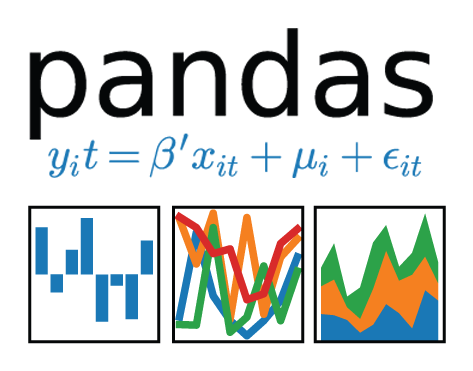
\includegraphics[scale=0.4]{./img/pandas-logo.png}
        \caption{Logo pandas}
        %        \label{}
    \end{figure}

    Pandas to biblioteka napisana w Pythonie służąca do manipulacji i analizy danych.
    Oferuje struktury danych, które ułatwiają operowanie na plikach csv, json i xlsx.
    Umożliwia operacje podobne do znanych z języka SQL.
    Są to: grupowanie danych, sortowanie po indeksie lub po innej kolumnie, łączenie tabel i usuwanie duplikatów.

    \section{Git}\label{sec:git}

    \begin{figure}[h]
        \centering
        
\includegraphics[scale=0.3]{./img/git-logo.png}
        \caption{Logo Gita}
        %        \label{}
    \end{figure}

    Git to rozproszony system kontroli wersji, czyli narzędzie do śledzenia zmian w plikach źródłowych.
    Jest to oprogramowanie używane głównie do zarządzania kodem, ale może być używane również do trzymania historii innych plików.
    Git ma na celu szybkość, spójność danych i wspieranie pracy rozproszonej wśród zespołów.
    Nie wymaga ciągłego dostępu do Internetu.
    Jest wykorzystywany w prawie wszystkich nowoczesnych projektach.

    Git został napisany przez Linusa Torvaldsa w 2005 roku, jako narzędzie do tworzenia jądra Linuksa, gdyż żaden inny system kontroli wersji nie spełniał jego wymagań.

    Główną strukturą w Gicie jest repozytorium.
    Każde repozytorium przypisane jest do jednego projektu.
    Posiada ono historię w formie grafu skierowanego, który jest drzewem.
    Git umożliwia poruszanie się po tym drzewie pozwalając przeglądać repozytorium w danym stanie.

    Praca z Gitem rozpoczyna się od sklonowania istniejącego repozytorium lub stworzenia nowego, pustego.
    Użytkownik po zmianie jakiegoś pliku śledzonego przez Gita może zrobić „commit”, czyli zapisać obecny stan projektu.
    Każdy „commit” ma przypisaną wiadomość, w której twórca „commita” informuje, co zmienił.
    Po „scommitowaniu” można zsynchronizować stan repozytorium z głównym serwerem.
    Dopiero wtedy inni użytkownicy mogą zobaczyć, jakie zaszły zmiany i pobrać do siebie najnowszą wersję.

    Git to potężne narzędzie, każdy programista powinien potrafić z niego korzystać.
    Łatwo jest poznać podstawy Gita i nie wymaga dużo czasu opanowanie ich.
    Zaawansowana znajomość Gita pozwala na robienie niesamowitych rzeczy w repozytorium.

    W projekcie inżynierskim korzystam z Gita do zapisywania postępów w tworzeniu aplikacji.
    Kod jest przechowywany na serwerze firmy GitHub.


    \section{Docker}\label{sec:docker}

    \begin{figure}[h]
        \centering
        
\includegraphics[scale=0.4]{./img/docker-logo.png}
        \caption{Logo Dockera}
        %        \label{}
    \end{figure}

    Docker to otwarto-źródłowe narzędzie służące do konteneryzacji aplikacji.
    Zapewnia dodatkową warstę abstrakcji nad systemem operacyjnym.
    Działa zarówno na Linuksie, jak i na Windowsie.
    Pierwsze wersje Dockera od 2013 roku napisane były w Pythonie, a kolejne w języku Go.

    W wielu aplikacjach Docker używany jest w celu ułatwienia wdrożenie aplikacji na serwery produkcyjne.
    Jest przydatny również w czasie wytwarzania dla deweloperów, gdyż idealnie nadaje się na środowisko testowe.

    Docker udostępnia na swojej stronie internetowej wiele predefiniowanych obrazów z zainstalowanymi aplikacjami, które są gotowe do użycia.
    Zalogowani użytkownicy mogą również publikować swoje własne obrazy zbudowane przez nich.
    Pozwala to dzielić się swoją pracą z całą społecznością.

    Praca z Dockerem polega na uruchomieniu kontenera z wybranego obrazu.
    Obraz dockerowy to tak jakby zapisany stan maszyny wirtualnej.
    Kontener jest konkretną uruchomioną instancją obrazu.

    Poza oficjalnymi obrazami, istnieje również możliwość tworzenia własnych obrazów do poszczególnych aplikacji.
    Polega to na stworzeniu pliku domyślnie o nazwie Dockerfile, gdzie podany jest obraz bazowy oraz lista komend do wykonania.
    Po zbudowaniu obrazu jedną komendą, można uruchomiać kontenery.

    W swoim projekcie inżynierskim korzystałem z Dockera, badania przeprowadzałem na serwerze, gdzie nie ma zainstalowanych wymaganych przeze mnie zależności.
    Dlatego to było jedynym rozwiązaniem.


    \chapter{Sieć neuronowa}\label{ch:siećNeuronowa}

    \section{Wprowadzenie}\label{sec:wprowadzenie}

    Sztuczna sieć neuronowa to pewna struktura matematyczna, która może być zaimplementowana programowo lub sprzętowo.
    Początkowo taki twórcy takich modeli inspirowali się zwierzęcym mózgiem, w którym połączone ze sobą neurony tworzą sieć.
    Taka sieć przetwarza sygnały wejściowe wykonując na nich pewne operacje.
    Sieci wykorzystywane są często do rozwiązywania problemów klasyfikacji, z racji na ich zdolność uczenia.
    Np. potrafią przetwarzać zdjęcia i opisywać, co się na nich znajduje.
    Przed skorzystaniem z sieci należy ją nauczyć, co sprowadza się do przekazywania na wejście sieci danych uczących razem z poprawną klasą, do której dane obiekty należą.

    \section{Neuron}\label{sec:neuron}

    \begin{figure}[h]
        \centering
        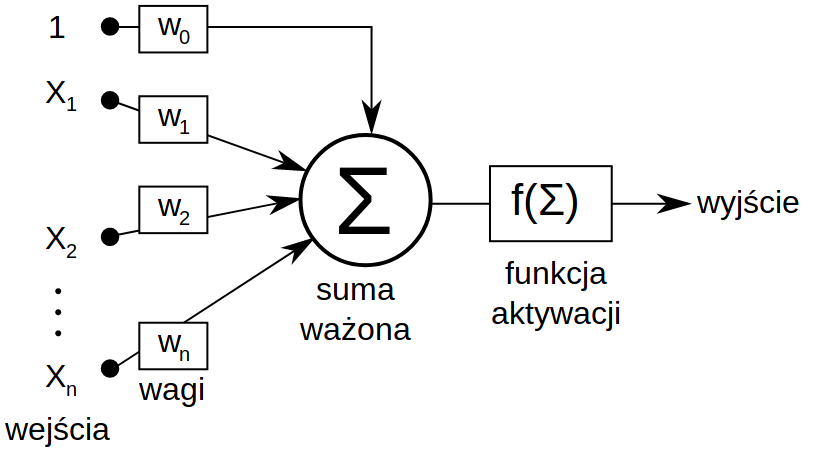
\includegraphics[scale=0.4]{./img/neuron.png}
        \caption{Schemat neuronu}
        %        \label{}
    \end{figure}

    \[
        s = \sum _{i=0}^{n} {w^{(i)} \cdot x^{(i)}} = w^T \cdot x
    \]

    Neuron stanowi podstawowy budulec sztucznej sieci neuronowej.
    Składa się z ustalonej liczby wejść, wraz z odpowiadającymi im wagami.
    Ponadto neuron zawiera nieliniową funkcję aktywacji oraz jedno wyjście.
    Jego zadanie to obliczenie iloczynu skalarnego wektora wejść z wektorem wag.
    Dodatkowo możemy przyjąć, że bias jest dodatkowym wejściem neuronu o wartości 1.
    Następnie obliczona suma ważona poddawana jest funkcji aktywacji i przekazywana na wyjście neuronu.
    W procesie uczenia wagi w neuronie zmieniają się tak, by wyliczona wartość funkcji błędu była jak najmniejsza.

    \subsection{Funkcja aktywacji}\label{subsec:funkcjaAktywacji}

    Funkcja aktywacji to funkcja, która wykorzystywana jest w sztucznych sieciach neuronowych, a dokładniej w samym neuronie do zmiany wartości wyjścia.
    Ma to na celu sprawienie, że sieć jest w stanie lepiej się uczyć nawet przy małej liczby neuronów.
    W uczeniu maszynowym znanych jest wiele rodzajów takich funkcji.
    W tej pracy opiszę tylko dwie, które użyłem do budowy sieci neuronowej.

    \[
        y = f(s) = f(w^T \cdot x)
    \]

    \subsubsection{Sigmoid}

    Pierwszą opisywaną funkcją jest sigmoid, zwana też „sigmoidalną funkcją unipolarną”.
    Bardzo dobrze nadaje się jako funkcja aktywacji, gdyż jej dziedzina to cały zbiór liczb rzeczywistych.
    Ma tę cechę, że zbiór warości mieści się w zakresie (0, 1).
    Jest to również wada, że szybko się „nasyca”.
    Kolejnym minusem tej funkcji jest to, że wartości nie zcentralizowane wokół zera.
    Ponadto wykorzystuje funkcję ekpotencjalną, która jest kosztowna obliczeniowo.
    Jej wzór to:
    \[
        \sigma(x) = \frac {1}{1+e^{-x}}
    \]

    \begin{figure}[h]
        \centering
        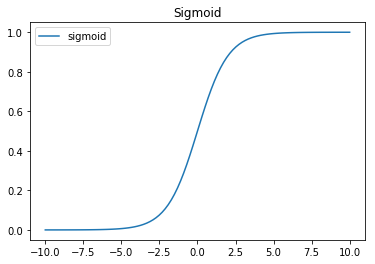
\includegraphics[scale=0.8]{./img/sigmoid.png}
        \caption{Funkcja aktywacji - sigmoid}
        %        \label{}
    \end{figure}

    \subsubsection{Tangens hiperboliczny}
    Kolejna funkcja, która wykorzystywana jest w sieciach neuronowych to tangens hiperboliczny (tanh).
    W tym przypadku również dziedziną jest zbiór liczb rzeczywistych.
    Spłaszcza wyjście w zakresie (-1, 1).
    Podobnie jak sigmoid szybko się „nasyca”.
    W przeciwieństwie do poprzedniej funkcji jest scentralizowany wokół zera.
    Tanh również korzysta z funkcji ekpotencjalnej.
    Jej wzór to:
    \[
        \tanh(x) = \frac {2}{1+e^{-2x}} - 1
    \]

    \begin{figure}[h]
        \centering
        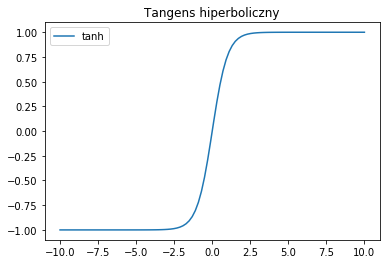
\includegraphics[scale=0.8]{./img/tanh.png}
        \caption{Funkcja aktywacji - tanh}
        %        \label{}
    \end{figure}

    \section{Model wielowarstwowy}\label{sec:modelWielowarstwowy}

    Kiedy pojedyncze neurony mają te same sygnały wejściowe, tworzą wówczas tak zwaną warstwę w sieci neuronowej.
    Dlatego sieć neuronowa ma budowę warstwową.
    Zawsze występuje warstwa wejściowa i wyjściowa.
    Ponadto mogą występować warstwy ukryte.
    Ich ilość zależy od rozwiązywanego problemu.

    \begin{figure}[h]
        \centering
        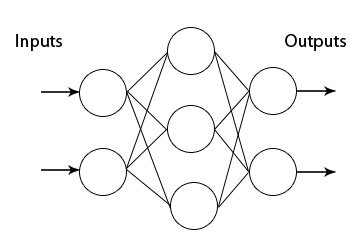
\includegraphics[scale=0.9]{./img/mlp.jpg}
        \caption{Schemat neuronu}
        %        \label{}
    \end{figure}

    W warstwie wejściowej znajduje się tyle neuronów, ile jest badanych cech.
    W moim przypadku będzie mniej niż 31.
    Neurony w tej warstwie nie mają wag, lecz przekazują dalej dokładnie to, co otrzymały.

    Liczba neuronów w warstwie wyjściowej również nie jest przypadkowa.
    Warstwa ta składa się z takiej samej liczby neuronów, co liczba klas w zadanym problemie.
    Problem medyczny, na którym pracuję dotyczy klasyfikacji ośmio klasowej, dlatego będzie osiem neuronów wyjściowych.
    Każdy z nich będzie zwracał wartość przynależności do danej klasy.

    \subsection{Proces uczenia}\label{subsec:procesUczenia}

    Uczenie sieci neuronowej, w którym znamy poprawne klasy dla danych uczących nazywamy uczeniem nadzorowanym lub uczeniem z nauczycielem.
    Polega na porównaniu wyjścia sieci z wartością oczekiwaną i dostrajaniu wag w neuronach tak, by minimalizować pewną ustaloną funkcję błędu.

    Korekcja wag odbywa się w procesie zwanym propagacją wsteczną.
    Propagacja wsteczna korzysta z gradientowych metod optymalizacji, które są wydajne obliczeniowo i bardzo skuteczne do uczenia sieci.
    Propagacja wsteczna wymaga również funkcję błędu.
    W tym celu stosuje się tak zwany „błąd średnio-kwadratowy”, który jest obliczany następująco:

    \[
        Q(w_k) = \sum_{k=1}^{N}{(d_k - y_k) ^ 2}
    \]

    gdzie:

    \begin{itemize}
        \item $Q$ - błąd średniokwadratowy,
        \item $w_k$ - wektor wag w k-tym neuronie,
        \item $N$ - liczba danych uczących,
        \item $d_k$ - poprawna wartość,
        \item $y_k$ - aktualna wartość,
    \end{itemize}

    Algorytm jest wieloetapowy.
    Pierwszym krokiem jest dostarczenie obiektu na wejście sieci i sprawdzenie jakie otrzymamy wyjście.
    Następnie rekurencyjnie zmniejszana jest wartość funkcji błędu od końca sieci zmieniając wagi w kolejnych warstwach.

    Tutaj korzysta się ze współczynnika uczenia.
    Na początku powinien mieć ustaloną wartość, a następnie wraz z kolejnymi epokami uczenia może się zmniejszać.

    Można to porównać do stania nad doliną górską, gdzie chcemy dość do najniższego punktu.
    Najpierw należy ustalić kierunek marszu, by później kroczyć w tym kierunku.
    Na początku kroki mogą być ogromne, ale w miarę schodzenia, powinniśmy je zmniejszać, by nie przekroczyć minimum.

    \chapter{Opis architektury aplikacji}\label{ch:opisArchitekturyAplikacji}

    \section{Schemat warstwy}\label{sec:schematWarstwy}

    \pythonexternal[caption={Schemat klasy Layer}]{./data/layer.py}

    Powyższy fragment kodu przedstawia schemat klasy Layer.
    Jest to implementacja jednej warstwy w sieci neuronowej.
    Przypomina schemat struktury danych zwanej listą dwukierunkową, gdyż zawiera referencje do poprzedniej i następnej warstwy.
    Klasa zawiera w sobie tablicę, która jest składa się z wag połączeń do poprzedniej warstwy.

    Przy tworzeniu instancji należy podać krotkę liczba oznaczającą kształt warstwy.
    Dodatkowo można przekazać nazwę funkcji aktywacji, którą domyślnie jest to sigmoid.

    Zadanie funkcji „feedforward” to przyjęcie tablicy liczb z poprzedniej warstwy, obliczenie iloczynu skalarnego z aktualnymi wagami i poddanie wyjścia funkcją aktywacji.
    Następnie funkcja powinna rekurencyjnie wywołać samą siebie na następnej warstwie jeśli nie jest ostatnia w sieci.
    W przeciwnym przypadku zwraca wyliczone wyjście całej sieci.

    Funkcja „calc\_delta” wywoływana jest rekurencyjne, ale w przeciwnym kierunku.
    Oblicza ona różnicę pomiędzy spodziewanym wyjściem warstwy a aktualnym.
    Pozwoli to później skorygować wagi każdej warstwy.

    Następna funkcja to „calc\_gradient”.
    Jest równnież wywoływana rekurencyjnie zaczynając od końca sieci.
    Oblicza wartość gradientu na podstawie wyjścia warstwy oraz wartości delty.

    Ostatnią funkcją jest „update\_weights”.
    Jak jej nazwa wskazuje, to właśnie ona zmienia wartości wag w warstwach odejmując iloczyn obliczonego gradientu ze współczynnikiem uczenia.
    W miarę uczenia współczynnik uczenia może się zmieniać, dlatego uznałem, że to dobre miejsce na dostarczenie tego współczynnika warstwie sieci neuronowej.

    \section{Tworzenie architektury sieci}\label{sec:tworzenieArchitekturySieci}

    \pythonexternal[caption={Schemat tworzenia sieci}]{./data/net.py}

    Funkcja „input\_data” tworzy pierwszą warstwę sieci neuronowej.
    Jako argument przyjmuje krotkę z wymiarem danych, które będą przekazywane do sieci.
    Ustawia w instacji warstwy, flagę informującą, że jest to warstwa wejściowa i zwraca ją.

    Druga ważna funkcja to „fully\_ connected”.
    Pierwszym argumentem, który należy jej podać to istniejąca już sieć neuronowa składająca się z połączonych rekurencyjnie warstw.
    „n\_units” to parametr, który jest liczbą neuronów w nowo utworzonej warstwie.
    Na koniec można podać, jaką funkcję aktywacji ma mieć ta warstwa.
    Gdy nie zostanie podana, to domyślnie będzie to „sigmoid”.
    Ta funkcja ustawia odpowiednie flagi w instancji warstwy i przypisuje wskaźniki do następników i poprzedników, jak w liście dwu kierunkowej.

    Kilka kolejnych linii kodu to proces tworzenia całej sieci neuronowej.
    Ta sieć przyjmuje 30 cech i może przypisać każdy obiekt do 8 klas.
    Pomiędzy wejściem a wyjściem znajdują się 3 warstwy ukryte o rozmiarach 24, 16 i 12 neuronów odpowiednio.
    Taka sieć jest gotowa przyjęcia danych i do nauki klasyfikacji.

    \section{Schemat modelu}\label{sec:schematModelu}

    \pythonexternal[caption={Schemat klasy Model}]{./data/model.py}

    Klasa Model jest nakładką na sieć neuronową.
    To z niej użytkownik aplikacji bezpośrednio korzysta.
    Model w inicjalizerze przyjmuje jeden argument - zaprojektowaną sieć neuronową.

    Funcja „fit” odpowiada za uczenienie sieci.
    Przyjmuje wiele argumentów w celu sprarametryzowania procesu.
    \begin{itemize}
        \item X\_inputs - tablica ze wszystkimi danymi uczącymi bez przypisanych im klas,
        \item Y\_targets - tablica zawierająca numery klas dla obiektów uczących,
        \item validation\_set - krotka zawierająca dane testowe,
        \item learning\_rate - krotka z 2 liczbami: współczynnikiem uczenia na początku i na końcu,
        \item n\_epoch - liczba określająca liczbę epoch,
        \item shuffle - flaga informująca o tym, czy dane uczące mają być pomieszane,
        \item train\_file - nazwa pliku w którym zapisywany jest postęp uczenia.
    \end{itemize}

    Metoda „fit” zbiera wszystkie możliwe dane z procesu uczenia, loguje je na konsolę i zapisuje do pliku.
    Dzięki temu możliwe jest przeprowadzenie badań i porównanie efektywności uczenia dla różnych wartości parametrów.

    Funkcje „predict” i „predict\_label” pozwalają skasyfikować wiele obiektów jednocześnie.
    Przyjmują tylko tablicę z wartościami cech.
    Jeśli potrzebne jest znać wsparcia wszystkich dla klas, to należy skorzystać z „predict”, a jeśli wystarczy informacja o najbardziej prawdopodobnej klasie, to można skorzystać z „predict\_label”.

    Ostatnie ważne funkcje to „save” i „load”.
    Obie potrzebują na wejściu nazwę pliku.
    Funkcja „save” zapisuje aktualne wagi do tego pliku w formie JSONa, a „load” wczytuje je ustawia wagi we wszyskich warstwach.
    Ważne jest, aby pamiętać, że architektura sieci musi się zgadzać.

    \chapter{Przeprowadzone badania}\label{ch:przeprowadzoneBadania}

    Do badań nad wpływem różnych parametrów na jakość klasyfikacji stworzyłem 120 różnych modeli sieci neuronowej.
    Modele te uczyły się na serwerze, który posiadał 30 CPU o nieznanych parametrach, z których wykorzystałem tylko 24 CPU.
    Ponadto serwer miał do dyspozycji 100 GB pamięci RAM.
    Czas uczenia wyniósł około 68 minut.

    Dodatkowo przeprowadziłem te same badania na innym serwerze posiadającym tylko 1 CPU i 4 GB pamięci RAM.
    Tutaj modelu uczyły się przez ponad 44 godziny.


    \begin{longtable}{|c|l|l|}
        \caption{Parametry uczenia sieci}\\ \hline
        \textbf{L.p.} & \textbf{Parametr} & \textbf{Wartości} \\ \hline
        \endfirsthead
        \multicolumn{3}{c}
        {\tablename\ \thetable\ -- \textit{Parametry uczenia sieci - c.d.}} \\ \hline
        \textbf{L.p.} & \textbf{Parametr} & \textbf{Wartości} \\ \hline
        \endhead
        \hline \multicolumn{3}{r}{\textit{Kontynuacja na następnej stronie}} \\
        \endfoot
        \hline
        \endlastfoot
        1 & architektura & \begin{tabular}[c]{@{}l@{}}
                               1) 24, 16, 12, 8\\ 2) 16, 12, 8\\ 3) 16, 8\\ 4) 8
        \end{tabular} \\ \hline
        2 & funkcja aktywacji & \begin{tabular}[c]{@{}l@{}}
                                    1) sigmoid\\ 2) tanh
        \end{tabular} \\ \hline
        3 & liczba cech & \begin{tabular}[c]{@{}l@{}}
                              1) 30\\ 2) 20\\ 3) 10
        \end{tabular} \\ \hline
        4 & współczynnik uczenia & \begin{tabular}[c]{@{}l@{}}
                                       1) od 0.2 do 0.2\\ 2) od 0.2 do 0.01\\ 3) od 0.2 do 0.001\\ 4) od 0.1 do 0.1\\ 5) od 0.1 do 0.01
        \end{tabular} \\
    \end{longtable}

    Parametr „architektura” informuje ile jest warstw ukrytych i ile zawierają one neuronów.
    Każda sieć na końcu ma 8 neuronów, ponieważ jest 8 możliwych klas.

    Do badań użyłem różnej liczby cech.
    Są to 30, 20 lub 10 cech o najwyższej wartości chi2.

    „Współczynnik uczenia” to dwie liczby, wartość na początku uczenia i na końcu.
    Jeśli jest powtórzona liczba, znaczy to, że był stały.
    W przeciwnym wypadku zmieniał się liniowo z każdą kolejną epoką.

    \begin{longtable}{|c|l|l|l|l|l|}
        \caption{Testowane modele}\\ \hline
        \textbf{L.p.} & \textbf{Nazwa} & \textbf{Architektura}  & \textbf{Funkcja aktywacji} & \textbf{Liczba cech} & \textbf{Współczynnik uczenia} \\ \hline
        \endfirsthead
        \multicolumn{5}{c}
        {\tablename\ \thetable\ -- \textit{Testowane modele - c.d.}} \\ \hline
        \textbf{L.p.} & \textbf{Nazwa} & \textbf{Architektura}  & \textbf{Funkcja aktywacji} & \textbf{Liczba cech} & \textbf{Współczynnik uczenia} \\ \hline
        \endhead
        \hline \multicolumn{5}{r}{\textit{Kontynuacja na następnej stronie}} \\
        \endfoot
        \hline
        \endlastfoot
        1 & $M_1$ & 24\_16\_12\_8 & sigmoid & 30 & 0.2\_0.2 \\ \hline
        2 & $M_2$ & 24\_16\_12\_8 & sigmoid & 30 & 0.2\_0.01 \\ \hline
        3 & $M_3$ & 16\_8 & sigmoid & 10 & 0.2\_0.001 \\ \hline
        4 & $M_4$ & 16\_8 & sigmoid & 20 & 0.2\_0.001 \\ \hline
        5 & $M_5$ & 16\_8 & sigmoid & 30 & 0.2\_0.001 \\ \hline
        6 & $M_6$ & 8 & sigmoid & 30 & 0.1\_0.01 \\ \hline
        7 & $M_7$ & 16\_8 & sigmoid & 30 & 0.1\_0.01 \\ \hline
        8 & $M_8$ & 16\_12\_8 & sigmoid & 30 & 0.1\_0.01 \\ \hline
        9 & $M_9$ & 24\_16\_12\_8 & sigmoid & 30 & 0.1\_0.01 \\
    \end{longtable}

    \section{Różne współczynniki uczenia}\label{sec:rozneWspolczynnikiUczenia}

    Poniżej znajduje się tabela z przebiegu uczenia dwóch modeli o architekturze 24\_16\_12\_8, funkcji aktywacji sigmoid, uczonym na 30 cechach i różniącym się współczynnikiem uczenia.


    \begin{longtable}{|c|l|l|l|l|}
        \caption{Porównianie modeli $M_1$ i $M_2$}\\ \hline
        & \multicolumn{2}{c|}{\textbf{$M_1$}} & \multicolumn{2}{c|}{\textbf{$M_2$}} \\ \hline
        \textbf{Epoka} & \textbf{Dokładność} & \textbf{Błąd}  & \textbf{Dokładność} & \textbf{Błąd} \\ \hline
        \endfirsthead
        \multicolumn{5}{c}
        {\tablename\ \thetable\ -- \textit{Porównianie modeli $M_1$ i $M_2$ - c.d.}} \\ \hline
        & \multicolumn{2}{c|}{\textbf{$M_1$}} & \multicolumn{2}{c|}{\textbf{$M_2$}} \\ \hline
        \textbf{Epoka} & \textbf{Dokładność} & \textbf{Błąd}  & \textbf{Dokładność} & \textbf{Błąd} \\ \hline
        \endhead
        \hline \multicolumn{5}{r}{\textit{Kontynuacja na następnej stronie}} \\
        \endfoot
        \hline
        \endlastfoot
        1 & 0.277 & 47.031 & 0.277 & 47.031 \\ \hline
        10 & 0.513 & 37.573 & 0.563 & 33.302 \\ \hline
        20 & 0.588 & 32.163 & 0.622 & 29.612 \\ \hline
        30 & 0.622 & 27.482 & 0.597 & 30.062 \\ \hline
        40 & 0.647 & 26.037 & 0.647 & 27.523 \\ \hline
        50 & 0.655 & 27.505 & 0.655 & 27.221 \\ \hline
        60 & 0.655 & 31.413 & 0.664 & 25.058 \\ \hline
        70 & 0.655 & 29.571 & 0.723 & 22.468 \\ \hline
        80 & 0.697 & 22.540 & 0.689 & 22.567 \\ \hline
        90 & 0.714 & 22.712 & 0.731 & 22.202 \\ \hline
        100 & 0.639 & 33.643 & 0.706 & 23.672 \\ \hline
        110 & 0.672 & 30.809 & 0.756 & 21.424 \\ \hline
        120 & 0.765 & 20.840 & 0.723 & 25.234 \\ \hline
        130 & 0.773 & 19.664 & 0.714 & 23.904 \\ \hline
        140 & 0.748 & 21.401 & 0.731 & 21.937 \\ \hline
        150 & 0.739 & 22.939 & 0.739 & 20.739 \\ \hline
        160 & 0.798 & 18.715 & 0.824 & 17.646 \\ \hline
        170 & 0.748 & 20.608 & 0.790 & 17.594 \\ \hline
        180 & 0.807 & 19.054 & 0.773 & 20.165 \\ \hline
        190 & 0.790 & 20.590 & 0.824 & 16.881 \\ \hline
        200 & 0.849 & 16.287 & 0.798 & 19.377 \\ \hline
        210 & 0.798 & 16.966 & 0.815 & 18.842 \\ \hline
        220 & 0.782 & 21.849 & 0.815 & 17.510 \\ \hline
        230 & 0.765 & 20.966 & 0.824 & 17.073 \\ \hline
        240 & 0.756 & 22.650 & 0.832 & 17.168 \\ \hline
        250 & 0.849 & 16.440 & 0.815 & 17.868 \\ \hline
        260 & 0.807 & 17.105 & 0.815 & 18.350 \\ \hline
        270 & 0.824 & 16.844 & 0.824 & 17.483 \\ \hline
        280 & 0.832 & 16.893 & 0.832 & 17.576 \\ \hline
        290 & 0.815 & 17.927 & 0.832 & 17.544 \\ \hline
        300 & 0.773 & 21.567 & 0.832 & 17.523 \\ \hline
        310 & 0.655 & 35.103 & 0.832 & 17.505 \\ \hline
        320 & 0.798 & 17.729 & 0.832 & 17.489 \\ \hline
        330 & 0.857 & 13.654 & 0.832 & 17.475 \\ \hline
        340 & 0.790 & 20.248 & 0.832 & 17.462 \\ \hline
        350 & 0.790 & 19.990 & 0.832 & 17.450 \\ \hline
        360 & 0.782 & 19.722 & 0.832 & 17.441 \\ \hline
        370 & 0.739 & 24.702 & 0.832 & 17.433 \\ \hline
        380 & 0.824 & 16.167 & 0.832 & 17.427 \\ \hline
        390 & 0.815 & 18.179 & 0.832 & 17.423 \\ \hline
        400 & 0.807 & 16.703 & 0.832 & 17.420 \\
    \end{longtable}

    Wykres wartości błędu przedstawia błąd średniokwadratowy z procesu uczenia co 5 epokę.
    Trend funkcji jest mniej więcej podobny, ale widać, że dla przypadku ze stałym współczynnikiem uczenia wartość błędu spada mniej gwałtownie.
    Gdy zmniejsza się współczynnik uczenia trening przebiega bardzo agresywnie, czasem daje chwilowo lepsze wyniki, ale przez większość epok błąd jet większy.

    \begin{figure}[h]
        \centering
        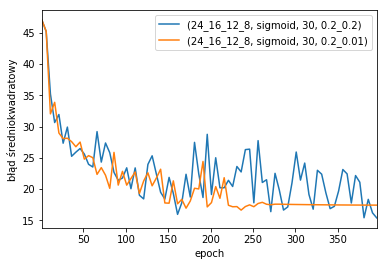
\includegraphics[scale=0.8]{./img/lr-error.png}
        \caption{Porównanie wartości błędu modeli $M_1$ i $M_2$}
        %        \label{}
    \end{figure}

    Dla wykresu porówniania dokładności można wysnuć podobne wnioski, że lepiej jest zmniejszać współczynnik uczenia w trakcie nauki.

    \begin{figure}[h]
        \centering
        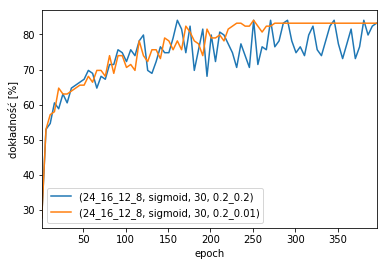
\includegraphics[scale=0.8]{././img/lr-accuracy.png}
        \caption{Porównanie dokładności modeli $M_1$ i $M_2$}
        %        \label{}
    \end{figure}

    Dzieje się tak dlatego, że po wielu epokach, gdy współczynnik uczenia dalej jest relatywnie duży gradient pomija minimum i zaczyna rosnąć.

    \section{Różna liczba cech}\label{sec:różnaLiczbaCech}

    Drugie porównanie to modele o architekturze 16\_8, funkcji aktywacji sigmoid.
    Trenowane były z malejącym współczynnikiem uczenia.
    Parametr, który je różni, to liczba cech.
    $M_3$ klasyfikuje korzystając z 10 cech o najwyższym współczynniku chi2.
    $M_4$ dostaje 20 cech, a $M_5$ uczy się na prawie wszystkich cechach, czyli 30 najlepszych.

    \begin{longtable}{|c|l|l|l|l|l|l|}
        \caption{Porównianie modeli $M_3$, $M_4$ i $M_5$}\\ \hline
        & \multicolumn{2}{c|}{\textbf{$M_3$}} & \multicolumn{2}{c|}{\textbf{$M_4$}} & \multicolumn{2}{c|}{\textbf{$M_5$}} \\ \hline
        \textbf{Epoka} & \textbf{Dokładność} & \textbf{Błąd} & \textbf{Dokładność} & \textbf{Błąd} & \textbf{Dokładność} & \textbf{Błąd} \\ \hline
        \endfirsthead
        \multicolumn{7}{c}
        {\tablename\ \thetable\ -- \textit{Porównianie modeli $M_3$, $M_4$ i $M_5$ - c.d.}} \\ \hline
        & \multicolumn{2}{c|}{\textbf{$M_3$}} & \multicolumn{2}{c|}{\textbf{$M_4$}} & \multicolumn{2}{c|}{\textbf{$M_5$}} \\ \hline
        \textbf{Epoka} & \textbf{Dokładność} & \textbf{Błąd} & \textbf{Dokładność} & \textbf{Błąd} & \textbf{Dokładność} & \textbf{Błąd} \\ \hline
        \endhead
        \hline \multicolumn{7}{r}{\textit{Kontynuacja na następnej stronie}} \\
        \endfoot
        \hline
        \endlastfoot
        1 & 0.538 & 41.299 & 0.496 & 41.714 & 0.462 & 43.907 \\ \hline
        10 & 0.571 & 34.109 & 0.613 & 26.876 & 0.613 & 28.462 \\ \hline
        20 & 0.647 & 29.445 & 0.714 & 24.232 & 0.655 & 23.769 \\ \hline
        30 & 0.664 & 27.188 & 0.723 & 20.451 & 0.765 & 20.308 \\ \hline
        40 & 0.672 & 26.045 & 0.782 & 17.584 & 0.765 & 18.426 \\ \hline
        50 & 0.681 & 23.634 & 0.782 & 16.687 & 0.824 & 15.077 \\ \hline
        60 & 0.739 & 21.233 & 0.790 & 16.759 & 0.849 & 14.902 \\ \hline
        70 & 0.773 & 20.575 & 0.832 & 15.302 & 0.849 & 13.756 \\ \hline
        80 & 0.765 & 22.901 & 0.849 & 14.367 & 0.874 & 12.665 \\ \hline
        90 & 0.739 & 21.739 & 0.849 & 13.351 & 0.866 & 12.680 \\ \hline
        100 & 0.765 & 21.240 & 0.857 & 13.708 & 0.857 & 12.414 \\ \hline
        110 & 0.739 & 20.959 & 0.832 & 14.686 & 0.874 & 11.797 \\ \hline
        120 & 0.756 & 20.595 & 0.866 & 13.803 & 0.874 & 11.426 \\ \hline
        130 & 0.773 & 20.562 & 0.874 & 12.516 & 0.882 & 11.068 \\ \hline
        140 & 0.798 & 20.210 & 0.874 & 12.519 & 0.891 & 10.854 \\ \hline
        150 & 0.798 & 19.903 & 0.866 & 13.173 & 0.899 & 10.735 \\ \hline
        160 & 0.798 & 19.924 & 0.882 & 12.943 & 0.908 & 10.647 \\ \hline
        170 & 0.807 & 19.784 & 0.866 & 13.364 & 0.908 & 10.576 \\ \hline
        180 & 0.807 & 19.581 & 0.849 & 13.898 & 0.908 & 10.529 \\ \hline
        190 & 0.815 & 19.234 & 0.849 & 14.285 & 0.908 & 10.507 \\ \hline
        200 & 0.807 & 18.782 & 0.849 & 13.564 & 0.908 & 10.536 \\ \hline
        210 & 0.798 & 18.772 & 0.849 & 13.768 & 0.908 & 10.761 \\ \hline
        220 & 0.782 & 18.848 & 0.857 & 13.938 & 0.874 & 11.259 \\ \hline
        230 & 0.765 & 19.123 & 0.857 & 13.972 & 0.882 & 10.923 \\ \hline
        240 & 0.773 & 18.967 & 0.866 & 13.971 & 0.908 & 10.914 \\ \hline
        250 & 0.790 & 18.496 & 0.866 & 13.969 & 0.908 & 10.813 \\ \hline
        260 & 0.790 & 18.480 & 0.866 & 13.976 & 0.899 & 10.745 \\ \hline
        270 & 0.798 & 18.272 & 0.866 & 13.991 & 0.899 & 10.722 \\ \hline
        280 & 0.807 & 18.269 & 0.857 & 14.007 & 0.891 & 10.729 \\ \hline
        290 & 0.798 & 18.229 & 0.857 & 14.019 & 0.891 & 10.752 \\ \hline
        300 & 0.798 & 18.170 & 0.857 & 14.027 & 0.891 & 10.780 \\ \hline
        310 & 0.807 & 18.101 & 0.857 & 14.034 & 0.891 & 10.808 \\ \hline
        320 & 0.807 & 18.028 & 0.857 & 14.040 & 0.891 & 10.834 \\ \hline
        330 & 0.807 & 17.961 & 0.857 & 14.043 & 0.891 & 10.858 \\ \hline
        340 & 0.815 & 17.909 & 0.857 & 14.043 & 0.891 & 10.880 \\ \hline
        350 & 0.815 & 17.824 & 0.857 & 14.042 & 0.891 & 10.899 \\ \hline
        360 & 0.815 & 17.725 & 0.857 & 14.040 & 0.891 & 10.917 \\ \hline
        370 & 0.815 & 17.647 & 0.857 & 14.038 & 0.891 & 10.933 \\ \hline
        380 & 0.807 & 17.589 & 0.857 & 14.035 & 0.891 & 10.948 \\ \hline
        390 & 0.807 & 17.545 & 0.857 & 14.032 & 0.891 & 10.962 \\ \hline
        400 & 0.807 & 17.523 & 0.857 & 14.032 & 0.891 & 10.972 \\
    \end{longtable}

    Z wykresu porównania wartości błędu uczenia tych modeli można wywnioskować, że liczba cech ma wpływ na jakość klasyfikacji.
    Im więcej cech, tym model popełnia mniejszy błąd.
    Od dwusetnej epoki błąd maleje bardzo wolno, dlatego można by przerwać wcześniej uczenie bez straty na jakości klasyfikacji.

    \begin{figure}[h]
        \centering
        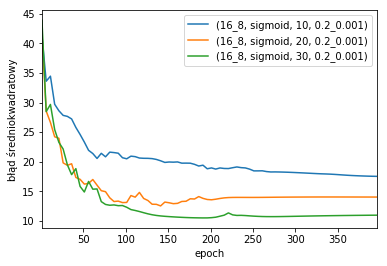
\includegraphics[scale=0.8]{./img/feat-error.png}
        \caption{Porównanie wartości błędu modeli $M_3$, $M_4$ i $M_5$}
        %        \label{}
    \end{figure}

    Wykres dokładności od epoki potwierdza, że dla tego zbioru danych warto użyć większej liczby cech, kosztem większego i bardziej skomplikowanego modelu.
    Tak jak na poprzednim wykresie, tutaj też po dwusetnej nie widać żadnej poprawy, a nawet obniżenie jakości predykcji może wskazywać na przeuczenie klasyfikatora.
    To znaczy, że za bardzo dostosował się do danych uczących tracąc zdolność do uogólniania.

    \begin{figure}[h]
        \centering
        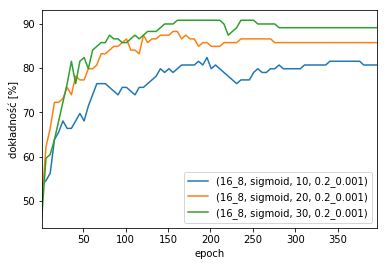
\includegraphics[scale=0.8]{././img/feat-accuracy.png}
        \caption{Porównanie dokładności modeli $M_3$, $M_4$ i $M_5$}
        %        \label{}
    \end{figure}

    \section{Różne architektury}\label{sec:różneArchitektury}

    Kolejnej analizie poddano sieci neuronowe mające funkcję aktywacji sigmoid oraz 30 neuronów w warstwie wejściowej.
    Współczynnik uczenia malał od $1.0$ do $0.01$ we wszystkich modelach tak samo.
    Kolejne klasyfikatory miały następujące architektury 8, 16\_8, 16\_12\_8 i 24\_16\_12\_8.

    Wydawać by się mogło, że im więcej warstw ukrytych, tym model dokonuje klasyfikacji z wyższą dokładnością.

    \begin{longtable}{|c|l|l|l|l|l|l|l|l|}
        \caption{Porównianie modeli $M_6$, $M_7$, $M_8$ i $M_9$}\\ \hline
        & \multicolumn{2}{c|}{\textbf{$M_6$}} & \multicolumn{2}{c|}{\textbf{$M_7$}} & \multicolumn{2}{c|}{\textbf{$M_8$}} & \multicolumn{2}{c|}{\textbf{$M_9$}} \\ \hline
        \textbf{Epoka} & \textbf{Dokładność} & \textbf{Błąd} & \textbf{Dokładność} & \textbf{Błąd} & \textbf{Dokładność} & \textbf{Błąd} & \textbf{Dokładność} & \textbf{Błąd} \\ \hline
        \endfirsthead
        \multicolumn{9}{c}
        {\tablename\ \thetable\ -- \textit{Porównianie modeli $M_6$, $M_7$, $M_8$ i $M_9$ - c.d.}} \\ \hline
        & \multicolumn{2}{c|}{\textbf{$M_6$}} & \multicolumn{2}{c|}{\textbf{$M_7$}} & \multicolumn{2}{c|}{\textbf{$M_8$}} & \multicolumn{2}{c|}{\textbf{$M_9$}} \\ \hline
        \textbf{Epoka} & \textbf{Dokładność} & \textbf{Błąd} & \textbf{Dokładność} & \textbf{Błąd} & \textbf{Dokładność} & \textbf{Błąd} & \textbf{Dokładność} & \textbf{Błąd} \\ \hline
        \endhead
        \hline \multicolumn{9}{r}{\textit{Kontynuacja na następnej stronie}} \\
        \endfoot
        \hline
        \endlastfoot
        1 & 0.361 & 54.950 & 0.420 & 45.093 & 0.387 & 46.705 & 0.420 & 45.093 \\ \hline
        10 & 0.630 & 28.059 & 0.605 & 28.339 & 0.563 & 33.505 & 0.605 & 28.339 \\ \hline
        20 & 0.647 & 28.050 & 0.655 & 26.151 & 0.630 & 29.422 & 0.655 & 26.151 \\ \hline
        30 & 0.697 & 26.420 & 0.723 & 22.149 & 0.647 & 27.208 & 0.723 & 22.149 \\ \hline
        40 & 0.681 & 27.203 & 0.756 & 19.402 & 0.672 & 25.992 & 0.756 & 19.402 \\ \hline
        50 & 0.697 & 26.257 & 0.824 & 16.846 & 0.697 & 24.958 & 0.824 & 16.846 \\ \hline
        60 & 0.697 & 26.023 & 0.832 & 15.827 & 0.681 & 23.236 & 0.832 & 15.827 \\ \hline
        70 & 0.706 & 25.647 & 0.832 & 15.026 & 0.681 & 22.635 & 0.832 & 15.026 \\ \hline
        80 & 0.714 & 25.314 & 0.840 & 14.182 & 0.714 & 22.061 & 0.840 & 14.182 \\ \hline
        90 & 0.723 & 24.919 & 0.840 & 13.757 & 0.748 & 21.656 & 0.840 & 13.757 \\ \hline
        100 & 0.731 & 24.451 & 0.840 & 13.870 & 0.756 & 20.421 & 0.840 & 13.870 \\ \hline
        110 & 0.723 & 24.131 & 0.849 & 13.930 & 0.773 & 19.475 & 0.849 & 13.930 \\ \hline
        120 & 0.731 & 23.937 & 0.840 & 13.729 & 0.748 & 18.962 & 0.840 & 13.729 \\ \hline
        130 & 0.723 & 24.139 & 0.840 & 13.372 & 0.765 & 18.062 & 0.840 & 13.372 \\ \hline
        140 & 0.714 & 24.308 & 0.840 & 13.044 & 0.756 & 18.048 & 0.840 & 13.044 \\ \hline
        150 & 0.714 & 24.331 & 0.840 & 12.807 & 0.756 & 18.073 & 0.840 & 12.807 \\ \hline
        160 & 0.723 & 24.246 & 0.849 & 12.668 & 0.782 & 17.879 & 0.849 & 12.668 \\ \hline
        170 & 0.731 & 24.122 & 0.849 & 12.622 & 0.782 & 17.810 & 0.849 & 12.622 \\ \hline
        180 & 0.739 & 23.974 & 0.849 & 12.606 & 0.790 & 17.619 & 0.849 & 12.606 \\ \hline
        190 & 0.739 & 23.798 & 0.849 & 12.606 & 0.807 & 17.330 & 0.849 & 12.606 \\ \hline
        200 & 0.739 & 23.590 & 0.857 & 12.630 & 0.815 & 17.058 & 0.857 & 12.630 \\ \hline
        210 & 0.748 & 23.349 & 0.857 & 12.693 & 0.815 & 16.827 & 0.857 & 12.693 \\ \hline
        220 & 0.748 & 23.076 & 0.857 & 12.782 & 0.815 & 16.665 & 0.857 & 12.782 \\ \hline
        230 & 0.748 & 22.790 & 0.857 & 13.083 & 0.807 & 16.587 & 0.857 & 13.083 \\ \hline
        240 & 0.748 & 22.544 & 0.849 & 13.245 & 0.807 & 16.578 & 0.849 & 13.245 \\ \hline
        250 & 0.765 & 22.413 & 0.849 & 13.167 & 0.815 & 16.604 & 0.849 & 13.167 \\ \hline
        260 & 0.748 & 22.411 & 0.857 & 13.130 & 0.815 & 16.627 & 0.857 & 13.130 \\ \hline
        270 & 0.731 & 22.462 & 0.849 & 13.109 & 0.824 & 16.603 & 0.849 & 13.109 \\ \hline
        280 & 0.731 & 22.496 & 0.840 & 13.083 & 0.815 & 16.538 & 0.840 & 13.083 \\ \hline
        290 & 0.739 & 22.517 & 0.840 & 13.056 & 0.815 & 16.464 & 0.840 & 13.056 \\ \hline
        300 & 0.748 & 22.535 & 0.840 & 13.031 & 0.815 & 16.395 & 0.840 & 13.031 \\ \hline
        310 & 0.748 & 22.553 & 0.840 & 13.008 & 0.815 & 16.340 & 0.840 & 13.008 \\ \hline
        320 & 0.739 & 22.572 & 0.849 & 12.986 & 0.815 & 16.305 & 0.849 & 12.986 \\ \hline
        330 & 0.739 & 22.591 & 0.849 & 12.966 & 0.815 & 16.291 & 0.849 & 12.966 \\ \hline
        340 & 0.731 & 22.608 & 0.849 & 12.947 & 0.815 & 16.294 & 0.849 & 12.947 \\ \hline
        350 & 0.731 & 22.622 & 0.857 & 12.930 & 0.815 & 16.310 & 0.857 & 12.930 \\ \hline
        360 & 0.731 & 22.633 & 0.857 & 12.916 & 0.815 & 16.335 & 0.857 & 12.916 \\ \hline
        370 & 0.731 & 22.639 & 0.857 & 12.906 & 0.815 & 16.367 & 0.857 & 12.906 \\ \hline
        380 & 0.731 & 22.641 & 0.857 & 12.900 & 0.815 & 16.407 & 0.857 & 12.900 \\ \hline
        390 & 0.731 & 22.640 & 0.857 & 12.897 & 0.815 & 16.454 & 0.857 & 12.897 \\ \hline
        400 & 0.731 & 22.636 & 0.866 & 12.898 & 0.815 & 16.509 & 0.866 & 12.898 \\
    \end{longtable}

    Wykres wartości błędu pokazuje, że bardziej skomplikowana architekrura wcale nie zapewnia lepszych wyników.
    Największy model $M_9$ przez prawie połowę okresu uczenia radził sobie najgorzej, a na koniec wyprzedził najmniejszy model $M_6$.

    Najlepsze wyniki osiągnięto z jedną warstwą ukrytą w modelu $M_7$, potem z dwoma warstwami ukrytymi $M_8$.

    \begin{figure}[h]
        \centering
        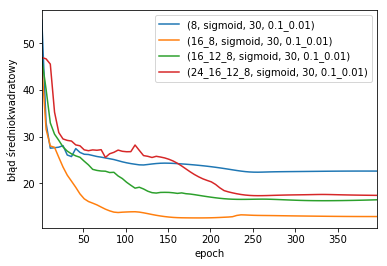
\includegraphics[scale=0.8]{./img/arch-error.png}
        \caption{Porównanie wartości błędu modeli $M_6$, $M_7$, $M_8$ i $M_9$}
        %        \label{}
    \end{figure}

    Zależność dokładności od epoki nie zmienia sytuacji.

    Ponownie można było przerwać uczenie w okolicy epoki numer 200, gdyż dalsze trenowanie nie poprawiało rezultatów.

    \begin{figure}[h]
        \centering
        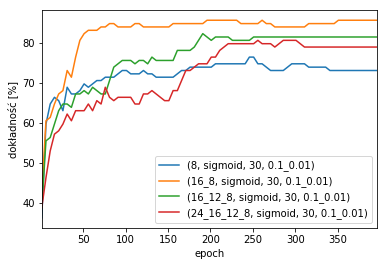
\includegraphics[scale=0.8]{./img/arch-accuracy.png}
        \caption{Porównanie dokładności modeli $M_6$, $M_7$, $M_8$ i $M_9$}
        %        \label{}
    \end{figure}

    \chapter{Podsumowanie}\label{ch:podsumowanie}

    \section{Dalsze możliwości rozwoju}\label{sec:dalszeMozliwosciRozwoju}

    \section{Co mogłem zrobić lepiej}\label{sec:coMoglemZrobicLepiej}

    Tekst podsumowania

    \bibliography{./bibliography}
    \bibliographystyle{plain}

    \listoffigures
    \listoftables

\end{document}
